\documentclass[12pt,a4paper]{report}
\usepackage[utf8]{inputenc}
\usepackage[T1]{fontenc}
\usepackage[brazil]{babel}
\usepackage{graphicx}
\usepackage{geometry}
\geometry{top=3cm, bottom=2cm, left=3cm, right=2cm}
\usepackage{setspace}
\usepackage{titlesec}
\usepackage{amsmath,amssymb}
\usepackage{url}
\usepackage{booktabs}
\usepackage[hidelinks]{hyperref}

% Ajuste de espaçamento dos títulos
\titleformat{\section}{\large\bfseries}{\thesection}{1em}{}

\begin{document}
\sloppy

% --- CAPA ---
\begin{titlepage}
    \begin{center}
        \setstretch{1.2}
        % --- LOGO AQUI ---
        \IfFileExists{figures/dccmapi_logo.pdf}{
\includegraphics[width=2.5cm]{figures/dccmapi_logo.pdf} \\}{\vspace*{2.5cm}} % Logo opcional
        \vspace{0.5cm}
        {\large \textbf{UNIVERSIDADE FEDERAL DO MARANHÃO}} \\
        {\large \textbf{UNIVERSIDADE FEDERAL DO PIAUÍ}} \\
        {\large \textbf{DOUTORADO EM CIÊNCIA DA COMPUTAÇÃO (DCCMAPI)}} \\

        \vspace{4.5cm}

        {\Large \textbf{ANTHONY IRLAN MARQUES LUZ}} \\

        \vspace{4.5cm}

        {\LARGE \textbf{RESPOSTAS: CAPÍTULO 1}} \\
        {\large \textit{REDES DE COMPUTADORES 5ed (TANENBAUM \& WETHERALL)}} \\

        \vfill

        \begin{flushright}
            \begin{minipage}{0.6\textwidth}
                \setstretch{1.1}
                Trabalho apresentado como requisito parcial para a disciplina de \textbf{Redes de computadores (PPGCC016)}, ministrada pelo \textbf{Prof. Dr. Rayner Gomes Souza}.
            \end{minipage}
        \end{flushright}

        \vfill

        {\large \textbf{PICOS -- PI}} \\
        {\large \textbf{2026}}

    \end{center}
\end{titlepage}

% --- CORPO DO TRABALHO ---
\newpage
\setstretch{1.5}
\pagenumbering{arabic}

\section*{Problemas}
\noindent \textbf{1:} Considere Bernie, um cachorro São Bernardo treinado para transportar uma caixa com três fitas de 8 mm. Cada fita armazena 7 GB de dados, e Bernie se desloca a 18 km/h. Determine para quais distâncias o transporte físico feito por Bernie apresenta uma taxa efetiva de dados superior à de uma linha de transmissão de 150 Mbps, desconsiderando overhead. Explique também como o resultado mudaria caso: (i) a velocidade de Bernie fosse duplicada; (ii) a capacidade de cada fita fosse duplicada; (iii) a taxa de transmissão da linha fosse duplicada. \\
\textbf{Resposta:}

As três fitas armazenam ao todo:
\[
    3 \times 7\,\text{GB}=21\,\text{GB}=168\,\text{Gb}.
\]
A velocidade de Bernie é \(18\,\text{km/h}=0{,}005\,\text{km/s}\). Para uma distância \(x\), em quilômetros, o tempo de deslocamento é
\[
    t=\frac{x}{0{,}005}=200x\,\text{s}.
\]
Logo, a taxa efetiva é
\[
    R=\frac{168}{200x}\,\text{Gbps}=\frac{840}{x}\,\text{Mbps}.
\]
Bernie supera a linha de \(150\,\text{Mbps}\) quando
\[
    \frac{840}{x}>150 \Rightarrow x<5{,}6\,\text{km}.
\]
Portanto, para distâncias menores que \(5{,}6\,\text{km}\), o transporte físico tem taxa efetiva superior. Se a velocidade de Bernie for duplicada, a distância limite também dobra, indo para \(11{,}2\,\text{km}\). Se a capacidade das fitas for duplicada, a distância limite também dobra. Se a taxa da linha for duplicada, a distância limite cai pela metade, ficando em \(2{,}8\,\text{km}\).

\vspace{0.6cm}

\noindent \textbf{2:} Uma possível alternativa ao uso de uma LAN seria utilizar um grande sistema de tempo compartilhado, com terminais conectados para todos os usuários. Apresente duas vantagens de uma arquitetura cliente-servidor baseada em LAN em comparação com essa solução centralizada. \\
\textbf{Resposta:}

Uma LAN pode crescer de forma incremental, com a adição gradual de computadores, servidores e dispositivos conforme a demanda aumenta. Além disso, ela distribui o poder de processamento entre várias máquinas, oferecendo interfaces interativas melhores e evitando a dependência completa de um único sistema central. Se os servidores forem replicados, uma falha isolada também não precisa derrubar todo o sistema. Em muitos cenários, essa solução ainda pode ser mais barata que um grande sistema centralizado de tempo compartilhado.

\vspace{0.6cm}

\noindent \textbf{3:} O desempenho de uma aplicação cliente-servidor depende, entre outros fatores, da largura de banda disponível e da latência da rede. Apresente um exemplo de rede que possua alta largura de banda, mas também alta latência. Em seguida, apresente um exemplo de rede com baixa largura de banda e baixa latência. \\
\textbf{Resposta:}

Um enlace transcontinental de fibra óptica é um exemplo de rede com alta largura de banda e alta latência: ele pode transportar muitos gigabits por segundo, mas a distância de milhares de quilômetros aumenta o atraso de propagação. Em contraste, um modem de \(56\,\text{kbps}\) conectado a outro computador no mesmo prédio teria baixa largura de banda, mas também baixa latência, pois a distância física percorrida pelo sinal seria pequena.

\vspace{0.6cm}

\noindent \textbf{4:} Além da largura de banda e da latência, indique outro parâmetro importante para avaliar a qualidade de serviço de uma rede nos seguintes tipos de tráfego: (i) voz digitalizada; (ii) vídeo; (iii) transações financeiras. \\
\textbf{Resposta:}

Para voz digitalizada e vídeo, outro parâmetro importante é o \textit{jitter}, isto é, a variação no atraso de entrega dos pacotes. Esses tráfegos precisam de entrega regular; atraso pequeno com grande variação pode ser pior que atraso um pouco maior, mas estável. Para transações financeiras, os parâmetros centrais são confiabilidade e segurança, pois é necessário evitar perda, alteração, interceptação ou falsificação das mensagens.

\vspace{0.6cm}

\noindent \textbf{5:} Em redes de comutação de pacotes do tipo \textit{store-and-forward}, parte do atraso ocorre porque cada switch precisa receber, armazenar e encaminhar o pacote. Considerando um tempo de comutação de \(10\,\mu s\), discuta se esse atraso seria relevante em uma comunicação cliente-servidor entre Nova York e Califórnia. Considere que a velocidade de propagação em meios como cobre e fibra óptica é aproximadamente \(2/3\) da velocidade da luz no vácuo. \\
\textbf{Resposta:}

Não. A velocidade de propagação em cobre ou fibra é cerca de \(200.000\,\text{km/s}\), isto é, \(200\,\text{m}/\mu\text{s}\). Em \(10\,\mu\text{s}\), o sinal percorre aproximadamente \(2\,\text{km}\). Assim, cada switch acrescenta atraso equivalente a apenas \(2\,\text{km}\) de cabo. Em uma distância da ordem de \(5000\,\text{km}\), mesmo 50 switches acrescentariam cerca de \(100\,\text{km}\) equivalentes, ou aproximadamente \(2\%\) do percurso. Portanto, nesse cenário, o atraso de comutação não é o fator principal; o atraso de propagação domina.

\vspace{0.6cm}

\noindent \textbf{6:} Considere um sistema cliente-servidor que utiliza comunicação via satélite, com o satélite localizado a uma altitude de 40.000 km. Determine o maior atraso possível para que uma solicitação seja respondida. \\
\textbf{Resposta:}

A solicitação precisa subir até o satélite e descer até o destino; a resposta faz o mesmo percurso no sentido inverso. O caminho total é:
\[
    4 \times 40.000\,\text{km}=160.000\,\text{km}.
\]
Como a velocidade da luz no ar ou no vácuo é aproximadamente \(300.000\,\text{km/s}\), o atraso mínimo de propagação é
\[
    \frac{160.000}{300.000}\approx 0{,}533\,\text{s}.
\]
Assim, o atraso apenas de propagação é de aproximadamente \(533\,\text{ms}\), sem contar filas, processamento ou retransmissões.

\vspace{0.6cm}

\noindent \textbf{7:} Imagine um cenário futuro em que todas as pessoas possuam terminais domésticos conectados a uma rede de computadores, permitindo consultas populares instantâneas sobre temas importantes. Embora esse modelo de democracia direta apresente vantagens evidentes, discuta possíveis consequências negativas desse tipo de sistema. \\
\textbf{Resposta:}

Um sistema de democracia direta instantânea poderia enfraquecer mecanismos tradicionais de deliberação, revisão e equilíbrio institucional. Muitas pessoas poderiam votar em questões complexas sem conhecer suficientemente os fatos, transformando opiniões pouco fundamentadas em decisões legais. Também haveria risco de manipulação por campanhas publicitárias de grupos de interesse. Outro problema sério seria a segurança: invasões, fraudes, manipulação de votos ou falhas no sistema poderiam comprometer a legitimidade das consultas populares.

\vspace{0.6cm}

\noindent \textbf{8:} Cinco roteadores devem ser interligados em uma sub-rede ponto a ponto. Para cada par de roteadores, pode-se escolher entre uma linha de alta velocidade, média velocidade, baixa velocidade ou nenhuma conexão. Sabendo que a geração e a análise de cada topologia levam 100 ms de processamento, calcule o tempo necessário para examinar todas as topologias possíveis. \\
\textbf{Resposta:}

Com cinco roteadores, há
\[
    \binom{5}{2}=10
\]
pares possíveis. Para cada par existem quatro possibilidades: linha de alta velocidade, média velocidade, baixa velocidade ou nenhuma linha. Logo, o número de topologias é
\[
    4^{10}=1.048.576.
\]
Como cada análise leva \(100\,\text{ms}=0{,}1\,\text{s}\), o tempo total é
\[
    1.048.576 \times 0{,}1 = 104.857{,}6\,\text{s}.
\]
Convertendo para horas:
\[
    \frac{104.857{,}6}{3600}\approx 29{,}13\,\text{h}.
\]
Portanto, seriam necessárias pouco mais de 29 horas.

\vspace{0.6cm}

\noindent \textbf{9:} Em uma sub-rede de broadcast, pode ocorrer desperdício de capacidade quando vários hosts tentam transmitir simultaneamente. Suponha que o tempo seja dividido em slots e que cada um dos \(n\) hosts tente acessar o canal com probabilidade \(p\) em cada slot. Determine a fração de slots desperdiçada devido a colisões. \\
\textbf{Resposta:}

Em um slot, a probabilidade de nenhum host transmitir é \((1-p)^n\). A probabilidade de exatamente um host transmitir com sucesso é \(np(1-p)^{n-1}\). Assim, a probabilidade de colisão, isto é, a fração de slots desperdiçada, é o complemento desses dois casos:
\[
    P_{\text{colisão}}=1-(1-p)^n-np(1-p)^{n-1}.
\]
Essa é a probabilidade de dois ou mais hosts tentarem transmitir simultaneamente no mesmo slot.

\vspace{0.6cm}

\noindent \textbf{10:} Explique duas razões que justificam a organização dos protocolos de rede em camadas. Em seguida, apresente uma possível desvantagem dessa abordagem. \\
\textbf{Resposta:}

Protocolos são organizados em camadas para dividir um problema complexo em partes menores e mais gerenciáveis. Outra vantagem é permitir que uma camada seja modificada internamente sem afetar as demais, desde que mantenha a mesma interface e o mesmo serviço oferecido. A principal desvantagem é a possível perda de desempenho, pois a separação em camadas adiciona cabeçalhos, processamento e restrições que um sistema monolítico altamente especializado talvez evitasse.

\vspace{0.6cm}

\noindent \textbf{11:} O presidente de uma empresa de tintas decide cooperar com uma cervejaria para desenvolver uma lata de cerveja invisível. A ideia passa pelo setor jurídico, depois pelos engenheiros das duas empresas, volta para os setores jurídicos e, por fim, retorna aos presidentes para discussão financeira. Considerando o modelo de protocolos em camadas, especialmente o modelo OSI, identifique qual princípio de comunicação em camadas é violado nesse processo. \\
\textbf{Resposta:}

O princípio violado é o de que, em um modelo em camadas, a comunicação física real não ocorre diretamente entre todas as camadas correspondentes. No modelo OSI, cada camada usa os serviços da camada inferior e oferece serviços à camada superior; a comunicação efetiva desce a pilha no transmissor, passa pelo meio físico na camada mais baixa e sobe a pilha no receptor. Portanto, o erro da analogia é imaginar que cada camada possa se comunicar fisicamente de forma direta e independente com sua camada correspondente.

\vspace{0.6cm}

\noindent \textbf{12:} Duas redes oferecem serviço confiável orientado à conexão. Uma delas fornece um fluxo confiável de bytes, enquanto a outra fornece um fluxo confiável de mensagens. Esses dois serviços podem ser considerados equivalentes? Justifique sua resposta e apresente um exemplo que mostre a diferença, caso ela exista. \\
\textbf{Resposta:}

Não. Em um fluxo de mensagens, os limites entre mensagens são preservados. Em um fluxo de bytes, esses limites se perdem, pois os dados são tratados como uma sequência contínua. Por exemplo, se um processo envia \(1024\) bytes e depois envia mais \(1024\) bytes, um serviço orientado a mensagens entregará duas mensagens separadas. Um serviço orientado a bytes pode entregar os \(2048\) bytes como uma única sequência, sem indicar que originalmente havia duas mensagens.

\vspace{0.6cm}

\noindent \textbf{13:} No contexto dos protocolos de rede, explique o significado do termo ``negociação''. Apresente também um exemplo de situação em que a negociação entre entidades de rede pode ocorrer. \\
\textbf{Resposta:}

Negociação é o processo pelo qual as partes envolvidas em uma comunicação concordam sobre parâmetros que serão usados durante a troca de dados. Um exemplo é a definição do tamanho máximo de pacote aceito. Outros exemplos incluem escolha de algoritmos de criptografia, parâmetros de compressão, controle de fluxo e opções de qualidade de serviço.

\vspace{0.6cm}

\noindent \textbf{14:} A Figura \ref{fig:relacionamento_servico_protocolo} apresenta um determinado serviço. Analise se existem outros serviços implícitos nessa figura. Caso existam, indique onde eles aparecem. Caso não existam, explique por quê. \\

\begin{figure}[h]
    \centering
    \IfFileExists{figures/q14.png}{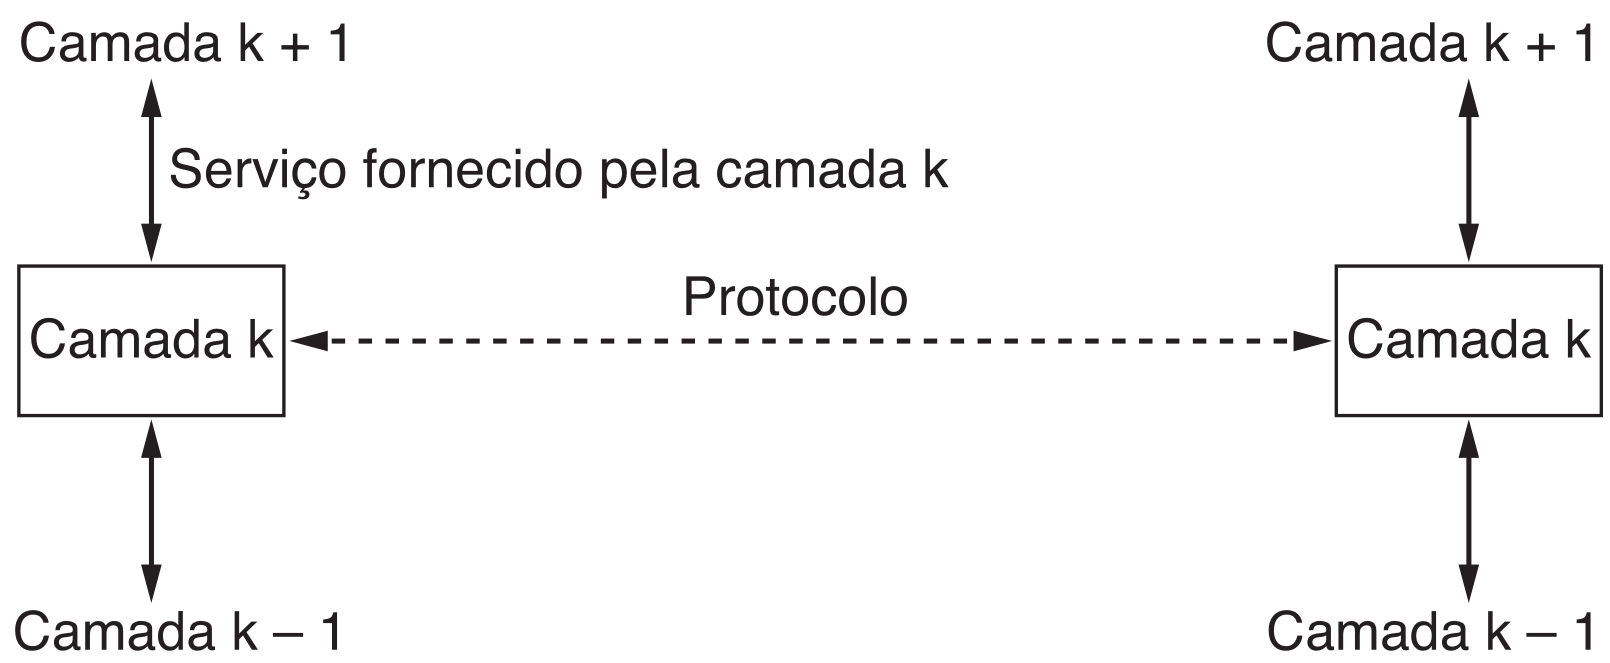
\includegraphics[width=0.5\textwidth]{figures/q14.png}}{\fbox{\parbox{0.45\textwidth}{\centering Figura não encontrada no diretório \texttt{figures/q14.png}.}}}
    \caption{Relacionamento entre um serviço e um protocolo.}
    \label{fig:relacionamento_servico_protocolo}
\end{figure}

\textbf{Resposta:}

A figura mostra o serviço oferecido pela camada \(k\) à camada \(k+1\). Há, porém, outro serviço implícito: o serviço oferecido pela camada \(k-1\) à camada \(k\). Portanto, a camada \(k\) é simultaneamente usuária do serviço da camada inferior e provedora de serviço para a camada superior.

\vspace{0.6cm}

\noindent \textbf{15:} Em algumas redes, a camada de enlace de dados lida com erros de transmissão solicitando a retransmissão de quadros corrompidos. Se a probabilidade de um quadro ser danificado é \(p\), determine o número médio de transmissões necessárias para que um quadro seja enviado corretamente. Considere que as confirmações nunca são perdidas. \\
\textbf{Resposta:}

A probabilidade de um quadro exigir exatamente \(k\) transmissões é a probabilidade de as \(k-1\) primeiras falharem e a \(k\)-ésima ter sucesso:
\[
    P_k=p^{k-1}(1-p).
\]
O número médio de transmissões é
\[
    E[K]=\sum_{k=1}^{\infty} k(1-p)p^{k-1}.
\]
Essa é a esperança de uma distribuição geométrica. Logo,
\[
    E[K]=\frac{1}{1-p}.
\]
Quanto maior for \(p\), maior será o número médio de transmissões necessárias.

\vspace{0.6cm}

\noindent \textbf{16:} Considere um sistema com uma pilha de protocolos formada por \(n\) camadas. As aplicações geram mensagens de \(M\) bytes, e cada camada acrescenta um cabeçalho de \(h\) bytes. Determine qual fração da largura de banda da rede é utilizada apenas para transmitir cabeçalhos. \\
\textbf{Resposta:}

Cada uma das \(n\) camadas acrescenta \(h\) bytes de cabeçalho. O total de cabeçalhos é, portanto, \(nh\). Como a mensagem original tem \(M\) bytes, o total transmitido é \(M+nh\). Assim, a fração da largura de banda usada apenas para cabeçalhos é
\[
    \frac{nh}{M+nh}.
\]

\vspace{0.6cm}

\noindent \textbf{17:} Explique a principal diferença entre os protocolos TCP e UDP. \\
\textbf{Resposta:}

O TCP é orientado à conexão, enquanto o UDP é não orientado à conexão. O TCP estabelece uma conexão lógica antes da troca de dados e fornece entrega confiável, ordenação, controle de fluxo e controle de congestionamento. O UDP envia datagramas sem estabelecimento prévio de conexão e sem garantir, por si só, entrega, ordem ou retransmissão.

\vspace{0.6cm}

\noindent \textbf{18:} A sub-rede apresentada na Figura \ref{fig:subrede_b} foi projetada com o objetivo de permanecer funcional mesmo diante de ataques severos. Considerando que cada bomba destrói um nó e todos os enlaces conectados a ele, determine quantas bombas seriam necessárias para dividir a rede em dois conjuntos de nós desconectados. \\

\begin{figure}[h]
    \centering
    \IfFileExists{figures/q18.png}{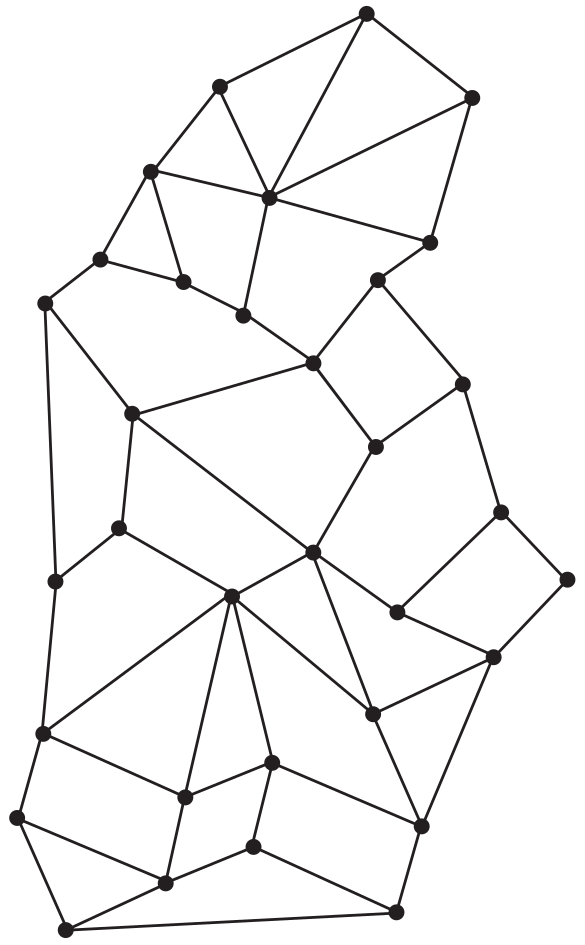
\includegraphics[width=0.3\textwidth]{figures/q18.png}}{\fbox{\parbox{0.30\textwidth}{\centering Figura não encontrada no diretório \texttt{figures/q18.png}.}}}
    \caption{Sistema distribuído de comutação proposto por Baran.}
    \label{fig:subrede_b}
\end{figure}

\textbf{Resposta:}

Na sub-rede indicada, os dois nós do canto superior direito podem ser isolados do restante da rede se forem destruídos os três nós aos quais estão conectados. Portanto, são necessárias três bombas para particionar a rede. A rede suporta a destruição de quaisquer dois nós sem se dividir em partes desconectadas.

\vspace{0.6cm}

\noindent \textbf{19:} Suponha que a Internet dobre de tamanho aproximadamente a cada 18 meses. Considerando a estimativa de 600 milhões de hosts em 2009, calcule o número previsto de hosts em 2018. Em seguida, discuta se esse resultado parece realista, justificando sua resposta. \\
\textbf{Resposta:}

De 2009 a 2018 há 9 anos. Como a Internet dobra a cada 18 meses, isto é, a cada 1,5 ano, há
\[
    \frac{9}{1{,}5}=6
\]
períodos de duplicação. O fator de crescimento é
\[
    2^6=64.
\]
Logo,
\[
    600.000.000 \times 64=38.400.000.000.
\]
A previsão seria de aproximadamente \(38{,}4\) bilhões de hosts. O valor parece alto para computadores tradicionais, mas é plausível quando se consideram celulares, televisores, câmeras, veículos, sensores e eletrodomésticos conectados.

\vspace{0.6cm}

\noindent \textbf{20:} Na transferência de um arquivo entre dois computadores, duas estratégias de confirmação podem ser usadas. Na primeira, o arquivo é dividido em pacotes, e cada pacote é confirmado individualmente. Na segunda, os pacotes não recebem confirmações individuais, mas o arquivo completo é confirmado ao final da transferência. Analise as vantagens e desvantagens dessas duas estratégias. \\
\textbf{Resposta:}

Confirmar cada pacote separadamente é melhor em redes com perdas, pois apenas os pacotes perdidos precisam ser retransmitidos. A desvantagem é a sobrecarga causada por muitas confirmações. Confirmar apenas o arquivo inteiro ao final economiza mensagens de controle em redes confiáveis, mas é ruim quando há perda: a perda de um único pacote pode exigir a retransmissão de todo o arquivo.

\vspace{0.6cm}

\noindent \textbf{21:} As operadoras de telefonia móvel precisam conhecer a localização aproximada dos aparelhos de seus assinantes. Explique por que essa característica pode ser prejudicial aos usuários. Em seguida, apresente razões pelas quais essa mesma característica pode ser benéfica. \\
\textbf{Resposta:}

A localização dos usuários pode prejudicar a privacidade, pois revela onde uma pessoa mora, trabalha, estuda, compra e se desloca. Esses dados podem ser vendidos, vazados, roubados ou usados para vigilância. Por outro lado, a localização também tem benefícios: permite direcionar socorro em emergências, ajuda a detectar fraudes e é necessária para o funcionamento técnico da rede móvel, como encaminhamento de chamadas e troca de células.

\vspace{0.6cm}

\noindent \textbf{22:} Calcule o comprimento físico de um bit, em metros, no padrão Ethernet 802.3 original. Considere uma taxa de transmissão de 10 Mbps e velocidade de propagação no cabo coaxial igual a \(2/3\) da velocidade da luz no vácuo. \\
\textbf{Resposta:}

A velocidade de propagação no cabo coaxial é aproximadamente \(200.000\,\text{km/s}\), ou \(200\,\text{m}/\mu\text{s}\). Em \(10\,\text{Mbps}\), o tempo de transmissão de um bit é
\[
    \frac{1}{10.000.000}\,\text{s}=0{,}1\,\mu\text{s}.
\]
Durante esse intervalo, o sinal percorre
\[
    200\,\text{m}/\mu\text{s}\times 0{,}1\,\mu\text{s}=20\,\text{m}.
\]
Logo, um bit tem aproximadamente \(20\,\text{m}\) de comprimento físico.

\vspace{0.6cm}

\noindent \textbf{23:} Uma imagem descompactada possui resolução de \(1600 \times 1200\) pixels e utiliza 3 bytes por pixel. Calcule o tempo necessário para transmiti-la pelos seguintes meios: modem de 56 kbps, modem a cabo de 1 Mbps, Ethernet de 10 Mbps, Ethernet de 100 Mbps e Gigabit Ethernet. \\
\textbf{Resposta:}

A imagem possui
\[
    1600\times 1200\times 3=5.760.000\,\text{bytes}=46.080.000\,\text{bits}.
\]
O tempo de transmissão é \(t=\frac{\text{bits}}{\text{taxa}}\). Assim:
\[
    \begin{array}{lcl}
        56\,\text{kbps}  & : & 822{,}857\,\text{s},                    \\
        1\,\text{Mbps}   & : & 46{,}080\,\text{s},                     \\
        10\,\text{Mbps}  & : & 4{,}608\,\text{s},                      \\
        100\,\text{Mbps} & : & 0{,}461\,\text{s},                      \\
        1\,\text{Gbps}   & : & 0{,}046\,\text{s}\approx 46\,\text{ms}.
    \end{array}
\]

\vspace{0.6cm}

\noindent \textbf{24:} Ethernet e redes sem fio possuem semelhanças e diferenças. Em uma rede Ethernet tradicional, apenas um quadro pode ser transmitido por vez no meio compartilhado. Analise se essa mesma propriedade também se aplica às redes sem fio do padrão 802.11. \\
\textbf{Resposta:}

Não necessariamente. Em uma Ethernet tradicional compartilhada, apenas um quadro deve ocupar o meio por vez. Em redes sem fio, o alcance limitado permite paralelismo espacial. Por exemplo, em uma sequência de estações \(A, B, C, D, E\), se cada estação alcança apenas suas vizinhas imediatas, \(A\) pode transmitir para \(B\) ao mesmo tempo em que \(D\) transmite para \(E\), sem interferência direta. Portanto, redes 802.11 não se comportam exatamente como uma Ethernet compartilhada clássica.

\vspace{0.6cm}

\noindent \textbf{25:} Apresente duas vantagens e duas desvantagens da adoção de padrões internacionais para protocolos de redes de computadores. \\
\textbf{Resposta:}

Duas vantagens dos padrões internacionais são interoperabilidade e economia de escala. Quando todos seguem o mesmo padrão, equipamentos de fabricantes diferentes conseguem se comunicar, e a produção em grande volume reduz custos. Duas desvantagens são a possibilidade de padrões tecnicamente ruins, resultantes de compromissos políticos, e a dificuldade de mudar um padrão depois que ele se torna amplamente adotado, mesmo quando surgem técnicas melhores.

\vspace{0.6cm}

\noindent \textbf{26:} Em sistemas compostos por uma parte permanente e uma parte removível, como ocorre com uma unidade de CD-ROM e o próprio disco, a padronização é importante para garantir compatibilidade entre produtos de fabricantes diferentes. Cite três exemplos, fora da área de informática, em que esse tipo de padronização internacional existe. Em seguida, cite três áreas, também fora da informática, nas quais essa padronização não está presente ou não é amplamente adotada. \\
\textbf{Resposta:}

Exemplos de padronização internacional fora da área de informática incluem contêineres marítimos ISO, cartões bancários utilizados em caixas eletrônicos e códigos de barras empregados no comércio. Esses casos ilustram situações em que a compatibilidade entre uma parte permanente e uma parte removível, ou entre produtos de diferentes fabricantes, depende de regras comuns amplamente aceitas.

Por outro lado, há áreas em que a padronização é ausente, incompleta ou não é adotada mundialmente. Entre os exemplos estão tomadas e plugues elétricos, que variam entre países; bitolas ferroviárias, que historicamente foram definidas de modo diferente em várias regiões; e sistemas de medidas, como o sistema métrico e o sistema imperial. Também podem ser citados o sentido de circulação no trânsito e diferentes padrões de tensão elétrica doméstica.

\vspace{0.6cm}

\noindent \textbf{27:} Suponha que os algoritmos internos usados para implementar as operações da camada \(k\) sejam alterados. Explique como essa mudança afeta, ou não, as operações das camadas \(k - 1\) e \(k + 1\). \\
\textbf{Resposta:}

Se apenas os algoritmos internos da camada \(k\) mudarem, sem alterar a interface nem o serviço oferecido, não há impacto nas camadas \(k-1\) e \(k+1\). A camada inferior continua oferecendo o mesmo serviço para \(k\), e a camada superior continua recebendo o mesmo serviço de \(k\).

\vspace{0.6cm}

\noindent \textbf{28:} Suponha agora que haja uma alteração no serviço oferecido pela camada \(k\), isto é, no conjunto de operações disponibilizadas por essa camada. Explique como essa mudança pode afetar os serviços das camadas \(k - 1\) e \(k + 1\). \\
\textbf{Resposta:}

Uma mudança no serviço oferecido pela camada \(k\) não afeta diretamente a camada \(k-1\), pois ela apenas fornece serviços para \(k\). Entretanto, afeta a camada \(k+1\), pois essa camada depende da interface e das operações oferecidas por \(k\). Se o serviço mudar, a camada superior precisará ser adaptada ou reimplementada.

\vspace{0.6cm}

\noindent \textbf{29:} Liste possíveis razões pelas quais o tempo de resposta observado por um cliente pode ser maior do que o atraso mínimo esperado no melhor caso. \\
\textbf{Resposta:}

O tempo de resposta pode ser maior que o mínimo esperado por perda ou corrupção de mensagens, exigindo retransmissões, ou por sobrecarga de processamento no servidor, satélite ou roteadores intermediários. Também podem contribuir congestionamento, filas, variação de rotas, controle de congestionamento e atrasos de processamento nas camadas de protocolo.

\vspace{0.6cm}

\noindent \textbf{30:} Explique quais são as principais desvantagens do uso de células pequenas e de tamanho fixo em redes ATM. \\
\textbf{Resposta:}

Células pequenas aumentam a sobrecarga relativa de cabeçalho, pois cada célula carrega seu próprio cabeçalho. Além disso, células de tamanho fixo podem desperdiçar espaço quando a carga útil não preenche completamente a célula, exigindo preenchimento. Assim, embora facilitem o processamento, podem reduzir a eficiência do uso da largura de banda.

\vspace{0.6cm}

\noindent \textbf{31:} Liste atividades cotidianas que dependem do uso de redes de computadores. Em seguida, discuta como sua rotina seria afetada caso essas redes deixassem de funcionar repentinamente. \\
\textbf{Resposta:}

Atividades cotidianas que dependem de redes incluem envio de mensagens, chamadas de vídeo, e-mail, acesso a sistemas acadêmicos e administrativos, pagamentos eletrônicos, operações bancárias, compras on-line, armazenamento em nuvem, streaming, mapas e transporte por aplicativo. Se essas redes parassem de funcionar, a comunicação ficaria mais lenta, pagamentos e autenticações seriam interrompidos, aulas e reuniões remotas seriam prejudicadas, sistemas institucionais ficariam inacessíveis e muitos serviços presenciais também seriam afetados, pois dependem de consulta e registro em rede.

\vspace{0.6cm}

\noindent \textbf{32:} Investigue quais redes são utilizadas em sua escola, universidade ou local de trabalho. Descreva os tipos de redes encontrados, suas topologias e os métodos de comutação empregados. \\
\textbf{Resposta:}

No meu ambiente de trabalho, identifiquei uma infraestrutura composta primordialmente por uma LAN cabeada (padrão Ethernet) para as salas administrativas e laboratórios, além de uma WLAN baseada no protocolo IEEE 802.11 (Wi-Fi) para dispositivos móveis e conectividade acadêmica.

A topologia física observada é a estrela estendida: os hosts finais e pontos de acesso (APs) convergem para switches de acesso localizados em racks setoriais, que por sua vez são interconectados a um switch core central por meio de fibra óptica (backbone). No topo da hierarquia, um roteador de borda gerencia a saída para a Internet por meio da RNP (Rede Nacional de Ensino e Pesquisa).

Em relação aos métodos de transferência de dados, a tecnologia predominante é a comutação de pacotes. Na camada de enlace, os switches realizam o encaminhamento de quadros Ethernet com base nos endereços MAC, enquanto na camada de rede, o roteamento de pacotes IP é gerenciado pelo roteador/firewall institucional, que também lida com VLANs para segmentar o tráfego administrativo do acadêmico.
\vspace{0.6cm}

\noindent \textbf{33:} Utilize o programa \texttt{ping} para enviar pacotes de teste a diferentes locais conhecidos e medir o tempo de ida e volta. A partir dessas medições, estime o tempo de percurso em uma única direção pela Internet em função da distância. Dê preferência a servidores de universidades, pois sua localização costuma ser conhecida com maior precisão, como Berkeley, MIT, Vrije Universiteit Amsterdam, University of Sydney e University of Cape Town. \\
\textbf{Resposta:}

Para estimar o tempo de percurso em uma única direção, utilizou-se a ferramenta de diagnóstico \texttt{ping} (com a flag \texttt{-c 4}) para mensurar o tempo de ida e volta médio (RTT) até os domínios especificados. A estimativa matemática do atraso de propagação unidirecional é dada por:
\[
    t_{\text{ida}} \approx \frac{RTT}{2}
\]

Foram utilizados os seguintes domínios institucionais: \url{https://www.berkeley.edu}, \url{https://www.mit.edu}, \url{https://www.vu.nl}, \url{https://www.sydney.edu.au} e \url{https://www.uct.ac.za}. Os resultados consolidados dessas aferições encontram-se sumarizados na Tabela \ref{tab:latencia_ping}.

\begin{table}[htpb]
    \centering
    \small
    \begin{tabular}{p{3.4cm}p{3.7cm}lcc}
        \toprule
        \textbf{Destino} & \textbf{Domínio utilizado} & \textbf{Localização} & \textbf{RTT (ms)} & \textbf{$t_{\text{ida}}$ (ms)} \\
        \midrule
        Berkeley & \url{www.berkeley.edu} & EUA & 56{,}45 & 28{,}23 \\
        MIT & \url{www.mit.edu} & EUA & 64{,}94 & 32{,}47 \\
        VU Amsterdam & \url{www.vu.nl} & Holanda & 243{,}17 & 121{,}59 \\
        University of Sydney & \url{www.sydney.edu.au} & Austrália & 352{,}13 & 176{,}07 \\
        University of Cape Town & \url{www.uct.ac.za} & África do Sul & Sem resposta & -- \\
        \bottomrule
    \end{tabular}
    \caption{Resultados das medições de latência (RTT) e estimativas do tempo de ida.}
    \label{tab:latencia_ping}
\end{table}

\textbf{Discussão dos resultados:}

Conforme evidenciado pelos dados da Tabela \ref{tab:latencia_ping}, observa-se uma tendência geral de aumento da latência em destinos geograficamente mais distantes, especialmente nos casos da Holanda ($243\,\text{ms}$) e da Austrália ($352\,\text{ms}$). A ausência de resposta por parte da \textit{University of Cape Town} pode estar associada a políticas de segurança da rede institucional, pois \textit{firewalls} e roteadores de borda frequentemente são configurados para descartar tráfego ICMP (\textit{Echo Requests}), evitando mapeamentos automatizados de rede e reduzindo a exposição a ataques.

Também é necessário observar com cautela os tempos de resposta referentes às instituições norte-americanas, Berkeley e MIT. Considerando que a origem das requisições foi o Brasil, mais especificamente Picos, Piauí, latências na ordem de $50$ a $60\,\text{ms}$ são baixas para uma comunicação direta até a Califórnia ou Massachusetts por enlaces transcontinentais. Essa discrepância sugere que as requisições podem ter sido atendidas por servidores de borda, mecanismos de cache, infraestrutura \textit{Anycast}, CDNs ou outros recursos de aproximação do conteúdo ao usuário. Portanto, os valores medidos por \texttt{ping} não necessariamente representam o atraso de propagação até os campi principais dessas universidades.
\vspace{0.6cm}

\noindent \textbf{34:} Acesse o site da IETF e verifique quais projetos estão em andamento. Escolha um projeto de seu interesse e escreva um relatório de aproximadamente meia página explicando o problema abordado e a solução proposta. \\
\textbf{Resposta:}

O projeto selecionado no âmbito da \textit{Internet Engineering Task Force} (IETF) é o trabalho relacionado ao protocolo QUIC (\textit{QUIC Transport Protocol}), que constitui uma base importante para comunicações modernas de baixa latência e para o HTTP/3 \cite{rfc9114}. O problema central enfrentado por essa linha de padronização está associado a limitações históricas da arquitetura baseada no TCP (\textit{Transmission Control Protocol}). Embora o TCP seja robusto e amplamente adotado, ele pode introduzir atrasos em aplicações interativas, principalmente por causa do \textit{Head-of-Line Blocking} (HoL Blocking), situação em que a perda de um pacote pode atrasar a entrega dos dados seguintes. Além disso, os \textit{handshakes} necessários para estabelecer conexões TCP e TLS podem aumentar o tempo inicial de comunicação, enquanto dispositivos intermediários da rede, conhecidos como \textit{middleboxes}, dificultam a evolução do protocolo de transporte \cite{rfc9000}.

Como solução, o QUIC implementa um transporte confiável e seguro sobre o UDP (\textit{User Datagram Protocol}). Essa escolha permite evoluir o protocolo no espaço de usuário, sem depender de alterações profundas no \textit{kernel} dos sistemas operacionais ou na infraestrutura intermediária da Internet. O QUIC também reduz o impacto do HoL Blocking ao oferecer multiplexação nativa de fluxos, de modo que a perda de dados em um fluxo não bloqueie necessariamente os demais. Outro ponto relevante é sua integração com o TLS 1.3, permitindo reduzir o custo de estabelecimento de conexão para 1-RTT ou, em conexões subsequentes, até 0-RTT \cite{rfc9001}. Assim, o projeto busca melhorar o desempenho, a segurança e a flexibilidade da comunicação na Internet, mantendo compatibilidade prática com a infraestrutura existente \cite{ietf_quic_wg}.

\vspace{0.6cm}

\noindent \textbf{35:} A Internet é formada por um grande conjunto de redes interconectadas, e sua organização define a topologia geral da rede. Pesquise informações sobre a topologia da Internet e escreva um breve relatório resumindo os principais aspectos encontrados. \\
\textbf{Resposta:}

A topologia da Internet pode ser compreendida como um grande sistema distribuído, formado pela interconexão de milhares de redes administradas de maneira independente. Essas redes são chamadas de Sistemas Autônomos (ASes) e são operadas por provedores de acesso, universidades, empresas, redes governamentais, provedores de conteúdo e outras organizações \cite{caida_itdk}. Tradicionalmente, essa organização foi descrita por meio de uma estrutura hierárquica em camadas, ou \textit{Tiers}. Nesse modelo, provedores de \textit{Tier 1} compõem uma espécie de \textit{backbone} global livre de trânsito pago (\textit{transit-free}); provedores de \textit{Tier 2} atuam no trânsito regional ou nacional; e provedores de \textit{Tier 3} ficam mais próximos dos usuários finais \cite{tanenbaum2011}.

O protocolo BGP (\textit{Border Gateway Protocol}) é o principal mecanismo usado para anunciar prefixos IP e estabelecer rotas entre esses diferentes Sistemas Autônomos \cite{rfc4271}. Entretanto, a Internet atual não pode ser descrita apenas como uma hierarquia rígida. Com o crescimento dos Pontos de Troca de Tráfego (IXPs --- \textit{Internet Exchange Points}) \cite{peeringdb} e das Redes de Distribuição de Conteúdo (CDNs), a topologia tornou-se mais achatada e mais interconectada. Em vez de todo o tráfego subir até grandes provedores de trânsito, muitos provedores de acesso e de conteúdo estabelecem conexões diretas de \textit{peering}, reduzindo custos, diminuindo latência e aproximando os dados dos usuários.

\vspace{0.6cm}

\noindent \textbf{36:} Pesquise alguns dos principais pontos de emparelhamento, ou \textit{peering points}, utilizados atualmente para o encaminhamento de pacotes na Internet. \\
\textbf{Resposta:}

No roteamento atual da Internet, os Pontos de Troca de Tráfego (IXPs --- \textit{Internet Exchange Points}), também chamados de \textit{peering points}, têm papel central na interconexão entre redes. Eles permitem que provedores de acesso, provedores de conteúdo, universidades, empresas e outras organizações troquem tráfego diretamente, sem depender sempre de provedores intermediários de trânsito. Na Europa, destacam-se o DE-CIX, em Frankfurt, e o AMS-IX, em Amsterdã, ambos historicamente reconhecidos pelo grande volume de tráfego e pela elevada quantidade de redes participantes \cite{ager2012anatomy}. O LINX (\textit{London Internet Exchange}), no Reino Unido, também é um ponto tradicional de interconexão, importante para o tráfego europeu e transatlântico.

Na América do Norte, a região de Ashburn, nos Estados Unidos, especialmente o ecossistema de datacenters da Equinix no chamado \textit{Data Center Alley}, é um ponto estratégico de interconexão, reunindo grande densidade de redes, provedores e serviços digitais \cite{lodhi2014}. Na América Latina, destaca-se o IX.br em São Paulo, operado pelo Núcleo de Informação e Coordenação do Ponto BR (NIC.br). Esse ponto de troca consolidou-se como uma das principais infraestruturas de interconexão da região, tanto em volume de tráfego quanto em quantidade de Sistemas Autônomos participantes \cite{ixbr_estatisticas}. A principal vantagem desses pontos é permitir o \textit{peering} direto entre redes, reduzindo caminhos desnecessariamente longos, diminuindo custos operacionais e melhorando a latência percebida pelos usuários \cite{chatzis2013}.

\vspace{0.6cm}

\noindent \textbf{37:} Escreva um programa que simule o fluxo de uma mensagem da camada superior até a camada inferior em um modelo de protocolo com sete camadas. O programa deve possuir uma função separada para cada camada. Cada função deve receber como parâmetros uma mensagem da camada superior e seu tamanho, acrescentar um cabeçalho de até 64 caracteres no início da mensagem, imprimir a nova mensagem na saída padrão e chamar a função correspondente à camada imediatamente inferior. A entrada do programa deve ser uma mensagem de aplicação com, no máximo, 80 caracteres. \\
\textbf{Resposta:}

Uma forma simples de resolver o problema é simular as sete camadas como sete funções distintas. Cada camada recebe a mensagem da camada superior, acrescenta seu próprio cabeçalho no início da mensagem, imprime o resultado e chama a camada imediatamente inferior.

\begin{verbatim}
programa SimuladorSeteCamadas

funcao adicionarCabecalho(nomeCamada, mensagem, tamanho)
    cabecalho <- "[" + nomeCamada + " | tam=" + tamanho + "] "

    // O cabeçalho gerado possui menos de 64 caracteres
    novaMensagem <- cabecalho + mensagem
    novoTamanho <- tamanho + comprimento(cabecalho)

    imprima(novaMensagem)

    retorne novaMensagem, novoTamanho
fim-funcao


funcao camada7_aplicacao(mensagem, tamanho)
    mensagem, tamanho <- adicionarCabecalho("Camada 7 - Aplicacao",
                                            mensagem, tamanho)
    camada6_apresentacao(mensagem, tamanho)
fim-funcao


funcao camada6_apresentacao(mensagem, tamanho)
    mensagem, tamanho <- adicionarCabecalho("Camada 6 - Apresentacao",
                                            mensagem, tamanho)
    camada5_sessao(mensagem, tamanho)
fim-funcao


funcao camada5_sessao(mensagem, tamanho)
    mensagem, tamanho <- adicionarCabecalho("Camada 5 - Sessao",
                                            mensagem, tamanho)
    camada4_transporte(mensagem, tamanho)
fim-funcao


funcao camada4_transporte(mensagem, tamanho)
    mensagem, tamanho <- adicionarCabecalho("Camada 4 - Transporte",
                                            mensagem, tamanho)
    camada3_rede(mensagem, tamanho)
fim-funcao


funcao camada3_rede(mensagem, tamanho)
    mensagem, tamanho <- adicionarCabecalho("Camada 3 - Rede",
                                            mensagem, tamanho)
    camada2_enlace(mensagem, tamanho)
fim-funcao


funcao camada2_enlace(mensagem, tamanho)
    mensagem, tamanho <- adicionarCabecalho("Camada 2 - Enlace",
                                            mensagem, tamanho)
    camada1_fisica(mensagem, tamanho)
fim-funcao


funcao camada1_fisica(mensagem, tamanho)
    mensagem, tamanho <- adicionarCabecalho("Camada 1 - Fisica",
                                            mensagem, tamanho)

    // A camada física é a última camada.
    // Portanto, ela apenas imprime a mensagem final.
fim-funcao


inicio
    imprima("Digite a mensagem da aplicacao: ")
    leia(mensagem)

    tamanho <- comprimento(mensagem)

    se tamanho > 80 entao
        imprima("Erro: a mensagem deve ter no maximo 80 caracteres.")
    senao
        camada7_aplicacao(mensagem, tamanho)
    fim-se
fim
\end{verbatim}

\bibliographystyle{abntex2-num}
\bibliography{referencias}
\end{document}